\section{Netzwerkkommunikation}
%________________________________________
\subsection{Kommunikationsarten und Protokolle}
\subsubsection{Verbindungslos \& Verbindungsorientiert}
\textbf{Verbindungsorientierte Kommunikation} zeichnet sich durch die folgenden Eigenschaften aus:
\begin{itemize}
    \item Die Verbindung zwischen Sender und Empfänger wir explizit durch einen Handshake aufgebaut.
    \item Die Übertragung von Paketen wird vom Empfänger bestätigt.
    \item Die Daten werden in der übergeordneten Schicht als verlustfreier geordneter Datenstrom wahrgenommen. Eine gesicherte Verbindung stellt nämlich sicher, dass Pakete ggf. erneut gesendet werden und in Ihrer Reihenfolge beim Empfänger sortiert werden.
    \item Broadcast und Multicast werden nicht unterstützt.
\end{itemize}
\textbf{Verbindungslose Kommunikation} zeichnet sich durch die folgenden Eigenschaften aus:
\begin{itemize}
    \item Es gibt keinen Verbindungsaufbau.
    \item Nachrichten werden ohne warten auf Antwort durch das Netzwerk gesendet.
    \item Die Reihenfolge der Pakete ist nicht garantiert.
    \item Es kann zu Paketverlusten kommen.
    \item Der Anwender muss die Reihenfolge und ggf. das erneute Senden von Nachrichten selbst managen.
\end{itemize}

\subsubsection{Synchrone und Asynchrone Kommunikation}
Je nach Szenario können synchrone oder asynchrone Kommunikation sinnvoll sein.\\
\textbf{Synchrone Kommunikation} zeichnet sich dadurch aus, dass das Senden und Empfangen von Nachrichten den Programmablauf blockiert. Möchte ein Sender also eine Nachricht senden, so würde er warten, bis das Senden möglich ist. Soll eine Nachricht empfangen werden, so wird so lange gewartet, bis die Nachricht eintrifft. Hier macht es Sinn mit Timeouts zu arbeiten.\\
\textbf{Asynchrone Kommunikation} zeichnet sich dadurch aus, dass das Senden oder Empfangen von Nachrichten nicht blockiert. Ein Sender würde also eine Nachricht versenden, egal, ob ein Empfänger bereit ist. Der Empfänger wartet nicht auf eine bestimmte Nachricht, sondern lässt sie puffern und liest sie dann, wenn er dafür bereit ist. Eventuell wird eine callback function aufgerufen, wenn das Event "Nachricht eingetroffen" eintrifft (z.B. über POSIX Signale).

\subsubsection{Qualitätsparameter von Netzwerken}
\begin{itemize}
    \item \textbf{Latenz:}\\
          Die minimale Verzögerung zwischen Sender und Empfänger. Also die Zeit, die benötigt wird, wenn man eine leere Nachricht versenden würde.
    \item \textbf{Datentransferrate:}\\
          Datenmenge, die innerhalb eines bestimmten Zeitraums maximal zwischen den Prozessen übertragen werden kann.
    \item \textbf{Nachrichtentransferzeit:}\\
          Die tatsächliche Verzögerung beim Versenden einer Nachricht. Sie setzt sich zusammen aus der Latenz und der Zeit, die für die pure Übertragung der Nachricht gebraucht wird:\\
          Latenz + Nachrichtenlänge / Datentransferrate
    \item \textbf{Durchsatz:}\\
          Menge der Bits, die pro Zeiteinheit über eine Verbindung übertragen werden.
    \item \textbf{Bandbreite:}\\
          Maximal möglicher Durchsatz des Netzwerks.
\end{itemize}

\subsubsection{Protokolle \& Internet}
Im Internet werden Daten übertragen, indem Sie mehrere logische Schichten und damit verbundene Protokoll durchlaufen (siehe OSI-\& TCP/IP-Modell).\\
Die Nachricht wird zunächst von der Anwendungsschicht aus mit puren Nutzdaten formuliert. Um diese Daten zu übertragen werden Protokolle benutzt, die sich dadurch auszeichnen, dass sie die Nachricht um Meta-Informationen erweitern und Regeln definieren, wie mit der Nachricht und den Protokollinformationen umgegangen werden soll. Ein paar Protokolle wollen wir hier noch kurz genauer betrachten:\\
\\
\textbf{IP - Internet Protokoll}\\
Das Internet Protocol ist die Implementierung der \textit{Internetschicht} (TCP/IP) bzw. \textit{Vermittlungsschicht} (OSI). Das IP bildet die Grundlage für alle relevanten Protokolle, die über das Internet Daten versenden möchten.\\
Das IP abstrahiert die verschiedenen möglichen Übertragungswege und Teilnetze, die im Internet existieren zu einem gemeinsamen Adressraum, der durch IP-Adressen definiert wird. Mittels dieser Form von Adressierung und Routing (der Wegfindung) kann mithilfe des IP eine Nachricht von einem Sender zu einem Empfänger gelangen.\\
Der Header des IP enthält vor Allem die Source- und Destination-IP-Address und eine TTL (Time to Live).\\
Das IP ist ein Verbindungsloses Protokoll, auf dessen Basis dann verbindungsorientierte Protokolle wie TCP arbeiten können.\\
\\
\textbf{UDP - User Datagram Protocol}\\
Das UDP ist eine Implementierung der Transportschicht (TCP/IP).\\
Das UDP verwendet Ports, um eine Nachricht dem richtigen Prozess auf dem Zielrechner zukommen zu lassen. Es erweitert also das IP von einer Rechner-Rechner Verbindung zu einer Prozess-Prozess verbindung. Außerdem können auch Checksums mitgesendet werden, um fehlerhaft Pakete beim Empfänger zu erkennen und zu verwerfen.\\
UPD ist eine sehr leichtgewichtiges verbindungsloses Protokoll, das benutzt wird, wenn Daten zeitkritisch ankommen müssen, aber Paketverluste nicht tragisch sind (z.B. Telefonie, Live-Streaming...).
Bei UDP entsteht wesentlich weniger Overhead als bei TCP, da keine Bestätigungen für Pakete gesendet werden.
UDP ist außerdem Broadcast und Multicast fähig. UDP ist grundsätzlich ein unidirektionales Protokoll, es kann jedoch in beide Richtungen gleichzeitig verwendet werden, um eine beidseitige Kommunikation zu erreichen.\\
\\
\textbf{TCP - Transmission Control Protocol}\\
Das TCP ist eine Implementierung der Transportschicht (TCP/IP).\\
TCP ist ein verbindungsorientiertes Protokoll. TCP benutzt auch, wie UDP, Ports als Adresszusatz. Die Kommunikation über TCP ist bidirektional. Multicasts oder Broadcasts sind mit TCP \textbf{nicht} auf einfache Weise möglich.\\
Beim TCP wird der Verbindungsaufbau durch einen 3 Wege Handshake eingeleitet. Danach werden Pakete versendet. Jedes Paket muss vom Empfänger bestätigt werden, jedoch können mehrere Pakete gleichzeitig bestätigt werden. Nicht bestätigte Pakete werden vom Sender nach gewisser Zeit erneut versendet. Der Verbindungsabbau wird wird ebenfalls mit einem 3-Wege-Handshake durchgeführt.\\
Der Header des TCP enthält im Wesentlichen die Ports beider Kommunikationspartner, eine Sequence-Number, welche die Reihenfolge der Pakete festlegt, eine Acknowledgement-Number, welche angibt welches TCP Paket als nächstes erwartet wird und eine Reihe von Options, die weitere kleinere Informationen übermitteln.\\
\\
\textbf{HTTP - Hypertext Transfer Protocol}\\
Das HTTP baut auf TCP auf. Bei TCP ist die Reihenfolge und das ankommen der Daten garantiert. Jedoch segmentiert TCP selbstständig die Daten als Pakete. Der Empfänger kann also zu keinem Zeitpunkt sicher sein, ob die Nachricht schon komplett eingetroffen ist, oder ob noch weitere TCP Pakete folgen. HTTP fügt TCP nun noch Header-Informationen hinzu, die unter anderem Anzeigen wie lang die Nachricht ist. Dadurch kann der Empfänger feststellen wann eine Nachricht endet und eine weitere Beginnt.

%________________________________________
\subsection{Sockets}
Sockets sind bidirektionale Kommunikationsendpunkte, die im Speicher als Objekt repräsentiert werden und vom Betriebssystem bereitgestellt werden. Sockets werden in fast allen Programmiersprachen unterstützt (C, C++, C\#, PHP...). Mittels Sockets kann ein Prozess mit einem anderen Kommunizieren. Mittels TCP- und UDP-Sockets kann die Kommunikation über Netzwerke erfolgen. D.h. der Kommunikationsmechanismus wird vom OS so bereitgestellt, dass ein Rechner mit einem Systemaufruf eine Nachricht an einen anderen Rechner senden kann, der diese mit einem Systemaufruf annehmen kann:\\

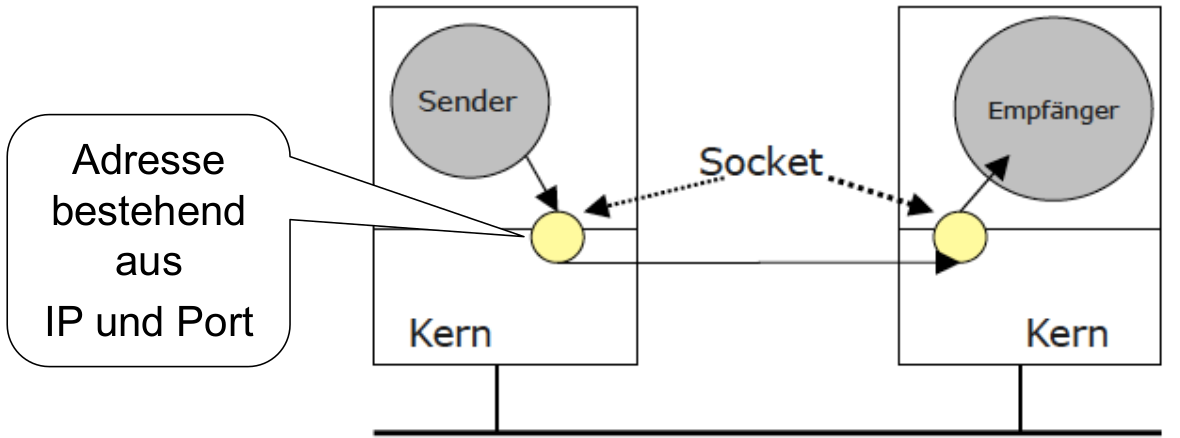
\includegraphics[width=10cm]{Sockets.png}

\subsubsection{UPD Sockets}
Das UDP ist zwar ein unidirektionales Protokoll, doch ein Socket-pair kann trotzdem bidirektional verwendet werden. Beide Empfänger benutzen dann jeweils UDP für eine Datenübertragung in eine Richtung aber über das gleiche Socket.\\
Bei der Benutzung von UDP Sockets wird durch einen Aufruf von \textit{send} genau ein Paket gesendet. Ist die Datenmenge zu groß, dann muss der Sender die Nachricht händisch in mehrere Pakete unterteilen.
Bei der Programmierung von UDP Sockets ist der Entwickler für folgendes verantwortlich:
\begin{enumerate}
    \item Senden jedes einzelnen Pakets (1 Paket bis 64kB)
    \item Korrektur der Reihenfolge der Pakete beim Empfänger
    \item Fehlerkorrektur
    \item Segmentierung großer Datenvolumen
\end{enumerate}
Für UDP stehen unter anderem folgende POSIX-Systemaufrufe zur Verfügung:
\begin{itemize}
    \item \textbf{socket} - Socket erzeugen
    \item \textbf{bind} - Socket an eine IP-Adresse binden
    \item \textbf{sendto}
    \item \textbf{recvfrom}
    \item \textbf{close}
    \item \textbf{setsockopt} - optionale Optionen (Puffergröße, REUSE\_ADDR, ...)
\end{itemize}

\newpage
\textbf{Hier ein Beispiel für die Programmierung mit UDP-Sockets:}\\

\textit{Code des Servers (Empfängers):}
\begin{lstinputlisting}[language=C++]
    {../src/UDP_receive/main.cpp}
\end{lstinputlisting}
\newpage
\textit{Code des Clients (Senders):}
\begin{lstinputlisting}[language=C++]
    {../src/UDP_send/main.cpp}
\end{lstinputlisting}


\subsubsection{TCP Sockets}
Die Benutzung von TCP erfordert im Gegensatz zur Benutzung von UDP zu Beginn der Kommunikation einen Verbindungsaufbau.\\
Der Server muss dafür seine IP Adresse und seinen Port  mit \textit{bind} an den Socket binden. Dann muss er mit \textit{listen} den Socket als passiven Socket markieren. Das bedeutet, dass er in der Zukunft über diesen Socket auf Anfragen warten möchte. Nun muss der Server \textit{accept} aufrufen. Accept blockiert so lange, bis eine Connection Request eines Clients eintrifft und gibt dann einen neuen Socket zurück, der mit dem Socket des Clients verbunden ist und zur Kommunikation genutzt werden kann. Der ursprüngliche Socket kann dann benutzt werden, um weitere Anfragen anzunehmen. Mit den Aufrufen \textit{send} und \textit{recv} können Sender und Empfänger bidirektional Daten versenden.\\
Ein wesentlicher Unterschied zwischen TCP und UDP ist, dass bei TCP eine beliebig große Menge an Daten mit einem Aufruf von send übertragen werden können. Der TCP Protokollstack kümmert sich dann um die Segmentierung der Daten. Das bedeutet, dass wir hier einen Datenstrom und nicht ein einzelnes Datenpaket übertragen. Für den Empfänger (Client) bedeutete das, dass er nicht wissen kann wie viele Pakete eintreffen und wann die Nachricht komplett übertragen wurde. Ein Aufruf von \textit{recv} gibt dann nicht wie bei UPD-sockets die Daten genau eines Aufrufes von \textit{send} zurück, sondern die Daten aller Pakete, die bisher eingetroffen sind. Diese Pakete können nur ein Teil einer Nachricht sein oder auch von mehreren separaten Nachrichten stammen. Daher benötigt man für eine sichere Anwendung mit TCP auch noch ein Format (z.B. HTTP), das spezifiziert wann eine Nachricht zu Ende ist und eine weitere Nachricht beginnt.\\
\\
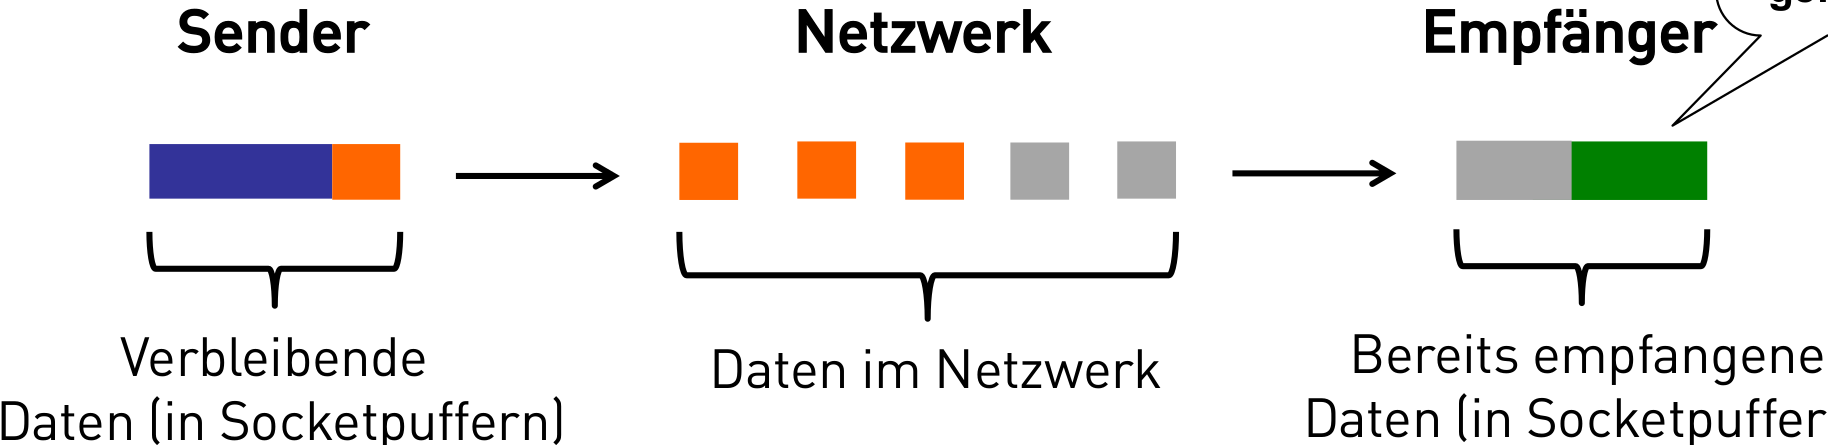
\includegraphics[width=11cm]{images/TCP_packets.png}
\\
\\
Für TCP Sockets stehen unter anderem folgende POSIX-Systemaufrufe zur Verfügung:
\begin{itemize}
    \item \textbf{socket} - Socket erzeugen
    \item \textbf{bind} - Socket an IP Adresse und Port binden
    \item \textbf{send}
    \item \textbf{recv}
    \item \textbf{connect} - wird vom client aufgerufen, um eine Verbindung zu initiieren
    \item \textbf{listen} - wird vom Server aufgerufen, um sein Socket als passives, also lauschendes Socket zu kennzeichnen
    \item \textbf{accept} - wird vom Server aufgerufen, um auf eine Verbindungsanfrage eines Clients zu warten
    \item \textbf{close}
\end{itemize}

\newpage
\textbf{Hier ein Beispiel für die Programmierung mit TCP-Sockets:}\\

\textit{Code des Servers:}
\begin{lstinputlisting}[language=C++]
    {../src/TCP_server/main.cpp}
\end{lstinputlisting}
\newpage
\textit{Code des Clients:}
\begin{lstinputlisting}[language=C++]
    {../src/TCP_client/main.cpp}
\end{lstinputlisting}

\subsubsection{Parallelisierung und \textit{select}}
Socketfunktionen \textit{connect}, \textit{accept}, \textit{send}, \textit{recv} arbeiten by default synchron und blockieren bis die Operation durchgeführt werden kann. Man bräuchte also n Threads, um eine Menge von n Sockets gleichzeitig zu Managen, obwohl die einzelnen Threads die meiste Zeit bloß blockiert sind und auf Aktivität warten. Es gibt mehrere Möglichkeiten dieses Problem zu beheben:\\
\textbf{Non Blocking Sockets}\\
Man kann Sockets aber auch beim Erzeugen in den Modus \textit{NONBLOCK} setzen, indem man die Funktion \textit{fcntl} mit dem Argument \textit{O\_NONBLOCK} für den Socket aufruft. Dann kehrt der Systemaufruf sofort zurück und der Rückgabewert gibt an, ob der Aufruf erfolgreich war.
So kann man also über eine Liste von Sockets iterireren und feststellen, ob einer der Sockets bereit für eine Aktion ist. So kann ein Prozess/Thread mehrere Sockets überwachen anstatt bei einem Socket dauerhaft blockert zu sein.\\
\textbf{Select}\\
Die Funktion \textit{select} setzt das gleiche Prinzip um. Ihr kann eine Liste von Sockets übergeben werden, die sie überwacht. Die Funktion blockiert bis einer der Sockets für die gewünschte Operation bereit ist. Dann kann man den gewünschten Socket finden und ihn bearbeiten. Bei der Nutzung von \textit{select} kann auch noch ein Optionaler Timeout angegeben werden.\\
Der Ablauf beim Benutzen von \textit{select} ist dann wie folgt:\\
\begin{enumerate}
    \item Alle Sockets mittels \textit{FD\_SET} in die eine Datenstruktur vom Typ \textit{fd\_set}(file descriptor set) eintragen.
    \item Die Funktion \textit{select} mit den Parametern aufrufen, die angeben auf welche Aktion man wartet.
    \item Nachdem select zurückgekehrt ist mittels \textit{FD\_ISSET} prüfen welcher Socket bereit ist.
    \item Diesen Socket bearbeiten (evtl. einen neuen Thread dafür erzeugen)
    \item Wieder bei 1. anfangen, um die Sockets neu in die Liste einzutragen, da \textit{select} destruktiv ist.
\end{enumerate}

\textbf{Hier ein kleines unvollständiges Beispiel:}\\

\begin{lstinputlisting}[language=C++]
    {../src/select_example.cpp}
\end{lstinputlisting}
\newpage

%________________________________________
\subsection{Remote Procedure Calls (RPC)}

Remote Procedure Calls sollen die Kommunikation über Sockets abstrahieren, die Komplexität verbergen und eine einfachere Schnittstelle für den Datentransfer über Netzwerke bereitstellen.
\subsubsection{Funktionsweise}
Es gibt eine Funktionssignatur (oder mehrere), also eine Schnittstelle, die auf Server- und Client-Seite gleich sein muss. Die Implementierung dieser Funktion befindet sich auf dem Server. Wenn der Client die Funktion aufruft soll nun der Server den Programmcode ausführen und den Rückgabewert zum Client zurückgeben. Für den Client soll es so aussehen, als hätte er eine lokale Funktion aufgerufen. Das läuft dann so ab:
\begin{enumerate}
    \item Der Client ruft die Funktion auf
    \item Das RPC Framework ruft eine sogenannte Stub-Funktion auf, die die Anfrage auf den Funktionsaufruf, sowie die Funktionsparameter serialisiert (Marshalling) und diese Daten über das Netzwerk via Sockets an den Server sendet
    \item Die Stub-Funktion auf dem Server wird übernimmt das Empfangen der Daten über den Socket und deserialisiert die Daten
    \item Die Implementierung der vom Client aufgerufenen Funktion wird mit den über das Netzwerk übermittelten Parametern ausgeführt.
    \item Eine Stub-Funktion des Servers serialisiert den Rückgabewert und sendet ihn über den internen Socket an den Client
    \item Die Funktion des Clients kehrt zurück, so als ob sie lokal (aber merkbar langsamer) ausgeführt worden wäre
\end{enumerate}

Die Implementierung der Stub-Funktionen, die die Abstrahierung der Datenübertragung schaffen, kommen von einem RPC-Framework. Es gibt viele RPC-Frameworks, alle implementieren das oben genannte Geschehen in ihrer eigenen Weise. Damit das Framework weiß an welchen Server der RPC gesendet werden soll, muss im Rahmen der Initialisierung auch noch die IP-Adresse und der Port des Servers angegeben werden. Bei der Initialisierung können je nach Framework auch noch zusätzliche Informationen angegeben werden, wie z.B.
\begin{itemize}
    \item Timeout bis das Warten auf den Rückgabewert des Servers abgebrochen wird
    \item Netzwerkprotokoll: UDP oder TCP, eventuell auch darauf aufbauend HTTP
    \item Datenformat: Binär, JSON, XML...
\end{itemize}

\subsubsection{Vorteile von RCP gegenüber Sockets}
\begin{itemize}
    \item Konkrete Aufrufe von Operationen über Sockets werden abstrahiert und vereinfacht
    \item Implementierung der Datenübertragung über Sockets wird einmalig durch RPC-Framework performant implementiert
    \item Konvertierung unterschiedlicher Zahlendarstellungen z.B. 1er vs. 2er Komplement, Big-Endian vs. Little Endian wird durch das Framework gewährleistet.
\end{itemize}

\subsubsection{Einschränkungen und Nachteile von RPC}
\begin{itemize}
    \item Bei Funktionsaufrufen kann kein call-by-reference und keine Übergabe mittels von Pointern erfolgen, weil der Adressraum des Callers nicht der gleiche Adressraum wie der des Ausführers der Funktion ist.
    \item Datenübertragung über RCP ist standardmäßig unverschlüsselt und kann abgehört werden
    \item Die Abstrahierung vereinfacht zwar die Datenübertragung für den Programmierer, aber man verliert dadurch natürlich auch Kontrolle über die Implementierung und die Analyse von Fehlern kann weniger präzise durchgeführt werden.
    \item RPC macht zwar den Aufruf der Funktionen auf dem Server durch das Verbergen der Sockets einfacher (\textit{Einfacher Zugriff auf Ressourcen}) aber in Bezug auf die anderen Qualitätsmerkmale Verteilter Systeme, \textit{Verteilungstransparenz, Offenheit, Skalierbarkeit, Zuverlässigkeit}, hilft uns RPC noch nicht wirklich weiter.
\end{itemize}

\subsubsection{Generelles Vorgehen bei der Programmierung mit RPCs}
Zunächst einmal stellt sich die Frage, woher der Code für die Stub-Funktionen kommt, die uns die Arbeit mit der Netzwerkübertragung vereinfachen. Dafür wird vom RPC-Framework eine Interface-Definition-Language (IDL) bereitgestellt, die i.d.R. auch für jedes Framework verschieden ist. Mithilfe dieser sehr einfachen Sprache definieren wir das Interface, also die Signaturen, der Funktionen, die über RPC erreichbar sein sollen. Das RPC-Framework stellt auch noch einen für die IDL spezifischen Compiler bereit, der aus der dem IDL-Code dann den \textbf{Source-Code} für die Stubs auf Server- und Clientseite generiert.
Das bedeutet also, dass die IDL gezielt als Cross-Platform Lösung designed ist, sodass der Source-Code der Stubs dann für beliebige Programmiersprachen generiert werden kann. Dieser Source-Code kann dann dann mit dem Source-Code des eigentlichen restlichen Programm zusammen kompiliert werden.\\

Die Generelle Vorgehensweise beim Programmieren mit einem RPC-Framework lässt sich wie folgt beschreiben:
\begin{enumerate}
    \item Die Funktionen der Schnittstelle auf dem Server implementieren
    \item Die Funktion an geeigneten Stellen im Code des Clients verwenden
\end{enumerate}

\textbf{Konkrete Implementierungen von RPC (RPC-Frameworks)}\\
\begin{itemize}
    \item \textbf{Sun ONC-RPC:} Das älteste und \quotes{originale} Framework, das nur die Sprache C unterstützt. Wird in diesem Dokument nicht genauer betrachtet
    \item \textbf{Apache Thrift:} Ein relativ modernes Framework, das viele Sprachen, wie C, C++, Java, PHP, Python u.v.m. unterstützt
    \item \textbf{Protocol Buffers - Protobuf:} Protocol Buffer ist ein Verfahren zur Serialisierung und Deserialisierung von Daten zu und von einem einheitlichen Format, das von Google entwickelt wurde. Das heißt beim Verwenden von Protobuf wird die Kommunikation noch vollständig vom Programmierer gelöst (also vermutlich über Sockets). Es ist also ein Datenformat, wie XML, das aber den Anspruch hat performanter und sparsamer zu sein.
    \item \textbf{gRPC:} ist ein modernes RPC-Framework von Google, das sehr ähnlich zu Apache Thrift ist, welches auf Protobuf basiert
    \item \textbf{XML-RPC:} Legt den Focus auf das Datenübertragungsformat, welches hier mittels XML läuft und dann über HTTP übertragen wird. Damit ist diese RPC Implementierung nicht besonders performant, aber sehr einfach, sodass sie auch leicht selbst mit einem HTTP-fähigen Server implementiert werden kann. Man muss nur aus dem XML ablesen welche Funktion aufgerufen werden soll und den Rückgabewert dann wieder als XML zurücksenden
    \item \textbf{JSON-RPC: } wie XML-RPC nur mit JSON
\end{itemize}

\subsubsection{Programmieren mit Apache Thrift}


Wir gehen schrittweise vor:\\
\\
\textbf{1. Definition des Interfaces in der IDL:}\\
Dazu erstellen wir das file \textit{example.thrift} mit einer einfachen Signatur einer Beispielfunktion, die zwei Zahlen addieren soll. Die Funktion \textit{ping} ist eine Funktion, die Serverseitig keine Implementierung bekommen soll. Sie soll sofort zurückkehren. Anhand ihrer Ausführungszeit kann man also ungefähr die Round-Trip-Time der RPC-Schnittstelle bestimmen.
\begin{lstinputlisting}[]
    {../src/RPC_Thrift/example.thrift}
\end{lstinputlisting}

Dabei wird ein Directory \textit{gen-cpp/} erstellt, das dann die Source Files für den Client, sowie ein Template für eine Implementierung auf Serverseite (Example\_server.skeleton.cpp) enthält. Alle files können im Ordner \textit{src/RPC\_Thrift/} dieses git-Repositories gefunden werden.\\
Das File für den Server können wir in ein anderes Directory kopieren und anpassen, vor allem die Implementierung der Funktion(en) des RPC-Interfaces ist natürlich notwendig. Die anderen generierten Files können wir so belassen, wie sie sind.\\
Wir werden feststellen, dass die generierten Dateien Bibliotheken includieren, die wir zuerst noch auf dem Host System installieren müssen. Dazu müssen wir das git-Repository clonen und die für die Installation erforderlichen Schritte durchführen. Wenn Thrift installiert ist werden die erforderlichen Dateien normalerweise unter \textit{/usr/local/include/thrift} abgelegt. Die Schritte zur Installation finden sich im Root-Verzeichnis dieses Repositories und sind zur Zeit folgende:

\begin{lstinputlisting}[]
    {../src/RPC_Thrift/docs/install-thrift-library.txt}
\end{lstinputlisting}

Das Programm muss dann mit den -lthrift Flag kompiliert werden. In dem Beispiel haben wir Example\_server.skeleton.cpp in das root directory verschoben und zu server-main.cpp umbenannt. Alle Files finden sich auch im \textit{src/RPC\_Thrift/} dieses Repositories. Simples Makefile:

\begin{lstinputlisting}[]
    {../src/RPC_Thrift/Makefile}
\end{lstinputlisting}

\textbf{3. Implementierung des Server-Codes:}\\
Die Implementierung des Servers ist sehr einfach, weil die Konfiguration schon im Code Template vorgegeben ist. Optional können wir hier noch den Port ändern. Wir müssen eigentlich also nur noch die tatsächliche Logik der Funktionen der Schnittstelle ergänzen. Diese Implementierung gestaltet sich bei unseren simplen Beispielfunktion natürlich sehr einfach (return a+b;). Hier nochmal das komplette Serverfile, das in \textit{src/RPC\_Thrift/server-main.cpp} zu finden:

\begin{lstinputlisting}[]
    {../src/RPC_Thrift/server-main.cpp}
\end{lstinputlisting}

\textbf{4. Implementierung des Client-Codes:}\\
Die Implementierung des Clients ist genau so simpel. Nur haben wir hier kein Template, sondern müssen selbst die Konfiguration vornehmen. Die ist aber im Grunde einfach und immer gleich, kann also kopiert werden. Wichtig ist natürlich nur den Server Namen und den Server Port anzupassen.\\
Nach der Konfiguration rufen wir die Funktion auf und schließen den Kanal wieder. Wir sollten uns bewusst sein, dass es sich um einen Funktionsaufruf handelt, der über Sockets kommuniziert wird. Daher müssen wir mit Verzögerungen und eventuell auch Exceptions rechnen. Der Code findet sich auch in \textit{src/RPC\_Thrift/client-main.cpp}:

\begin{lstinputlisting}[]
    {../src/RPC_Thrift/client-main.cpp}
\end{lstinputlisting}

\textbf{5. Starten}\\
Dazu muss der Source-Code, wie in \textit{src/RPC\_Thrift/Makefile} angegeben, kompiliert werden. Dann sollte zuerst der Server und dann der Client gestartet werden.